I will now discuss the results of my implementation of the algorithm and the implemented Hamiltonians.
The code is written in Python, while for the semidefinite program the interface picos is used.
To produce informative plots, the implementation executes the algorithm, with output $y$, and computes the ratio $r=\frac{y^{T}Cy}{\lambda_{max}}$ $o$ times per number of qubits $n$.
The average of the $o$ ratios per $n$ is plotted, whereas a logarithmic scale is used for the $x$-axis.
I have chosen to plot in the range of $n=4$ to $n=5200$ in equidistant steps on the logarithmic scale, using $o=20$. \todo{say that computation time was too high for higher n?}

The Ising model with a transverse field has physical relevance because it can be used to study quantum phase transitions of ferroelectrics with a tunneling effect or systems of interacting magnetic spins with an outer field.
The Hamiltonian,
\[
H=\alpha \sum_{i} Z_i + \beta \sum_{i} X_iX_{i+1}
\]
has been exactly solved in one dimension in \cite{pfeuty70}.
One way to do this by transforming the Hamiltonian into a quadratic form of Fermi operators and diagonalize it. \todo{should i describe it in detail?}
The parameter $\alpha$ corresponds to the tunneling energy and $\beta$ to the nearest neighbour interaction.
We here look at a closed chain, meaning $1\le i \le n, \quad X_{n+1}=X_{1}$.
I have first implemented the model with $\alpha =0, \quad \beta =1$.
This is a model of a one-dimensional chain with nearest neighbor interaction with out an outer field.
The state that is stabilized by all terms simultaneously is the state achieving the maximal eigenvalue.
In this case, it is the $n$-fold tensor product of the $+1$-eigenvector of $X$: \[
\ket{\psi}= \ket{+X_1}\otimes\ldots\otimes\ket{+X_n}
,\] where \[
\ket{+X_i}= \frac{\ket{0}_i+\ket{1}_i}{\sqrt{2}}
.\]
The maximal eigenvalue of the Hamiltonian is therefore $\lambda_{max}=n$, since it has $n$ terms.
\begin{figure}[H]
	\centering
	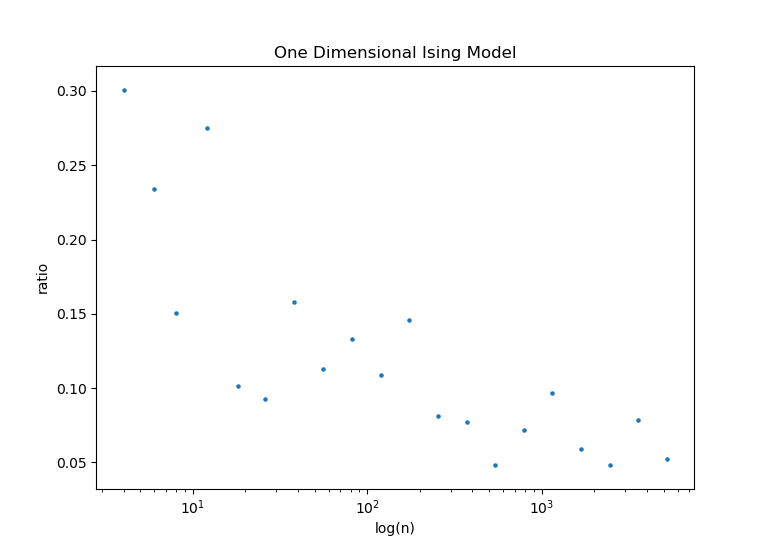
\includegraphics[width=0.9\textwidth]{avgchainplotn(4,5200,2,20,20)}
	\caption{blablabla}
	\label{fig:1}
\end{figure}
Fig. 1 is the result of my implementation of this model.
It exhibits the expected behaviour of $\Omega(\frac{1}{\log{}n})$.
I have also implemented the transverse field Ising model for non-zero $\alpha$.
Since this Hamiltonian has terms that are linear in Pauli operators, we have to transform it as discussed in chapter 4.
The Hamiltonian that was implemented is \[
H = H_2 + Z_{n+1}H_1 =\alpha Z_{n+1}\sum_{i} Z_i + \beta \sum_{i} X_iX_{i+1}
.\]
Fig. 2 shows the result of implementing this model.
\begin{figure}[H]
	\centering
	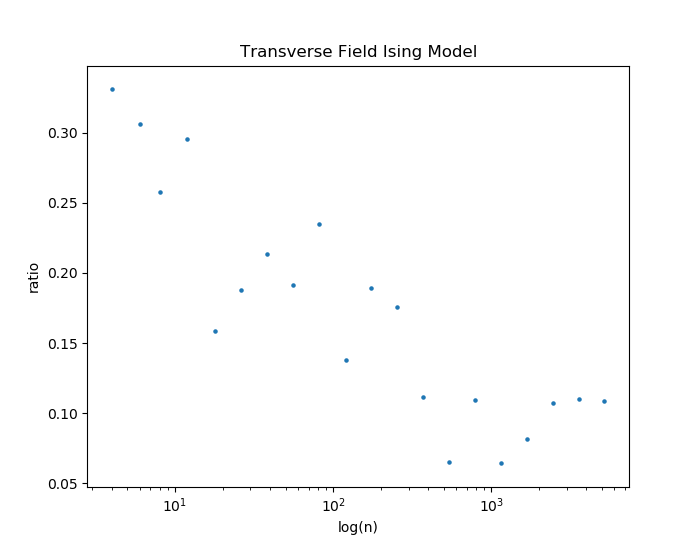
\includegraphics[width=0.9\textwidth]{tfiplot(4,5200,2,20,20,2,3)}
	\caption{lalala}
	\label{fig:2}
\end{figure}
The second Hamiltonian implemented is \[
	H = \sum_{i=1}^{\frac{n}{4}} X_iX_{i+1}+Z_iZ_{i+1}+X_{i+2}+X_{i+3},
\]
where we restrict $n$ to be a multiple of $4$.
In contrast to the Ising model without a transverse field, the maximal eigenvalue can not be achieved by a product state in this case.
To find out the maximal eigenvalue lets look at the first two quadratic terms:
\[
H_2=X_1X_2+Z_1Z_2
.\]
The state achieving the maximal eigenvalue $\lambda_{max}(H_2)=2$ is the EPR-state $\ket{\text{EPR}}=\frac{\bra{00}+\bra{11}}{\sqrt{2}}$
This is a maximally entangled state.
To find out the product state which approximates this the best, look at a general product state and maximize the overlap.
\[
	\ket{\psi}=\ket{\psi_1}\otimes\ket{\psi_2}=\left(a_1\ket{0}+b_1\ket{1}\right)\otimes\left(a_2\ket{0}+b_2\ket{1}\right)
\] with $a_1^2+b_1^2=a_2+b_2^2=1$.
\[
\max_{\psi_1,\psi_2}\left(\left|\braket{\text{EPR}}{\psi}\right|^2\right)=\max\left(\left|\frac{1}{\sqrt{2}}\left(a_1a_2+b_1b_2\right)\right|^2\right)=\frac{1}{2}
\]
with either $a_1=a_2=1$ and $b_1=b_2=0$ or $b_1=b_2=1$ and $a_1=a_2=0$.
Therefore, the product states with the maximal overlap are $\ket{00}$ and $\ket{11}$ with maximal eigenvalue $\lambda_{sep}(H_2)=1$, the approximation ratio being  $\frac{\lambda_{sep}H(2)}{\lambda_{max}(H_2)} = 0.5$.\\
In general the maximal product state of the Hamiltonian is therefore $\lambda_{max}(H)=n$, and the best achievable eigenvalue by a product state is $\lambda_{sep}(H)\frac{3}{4}n$.
\begin{figure}[H]
	\centering
	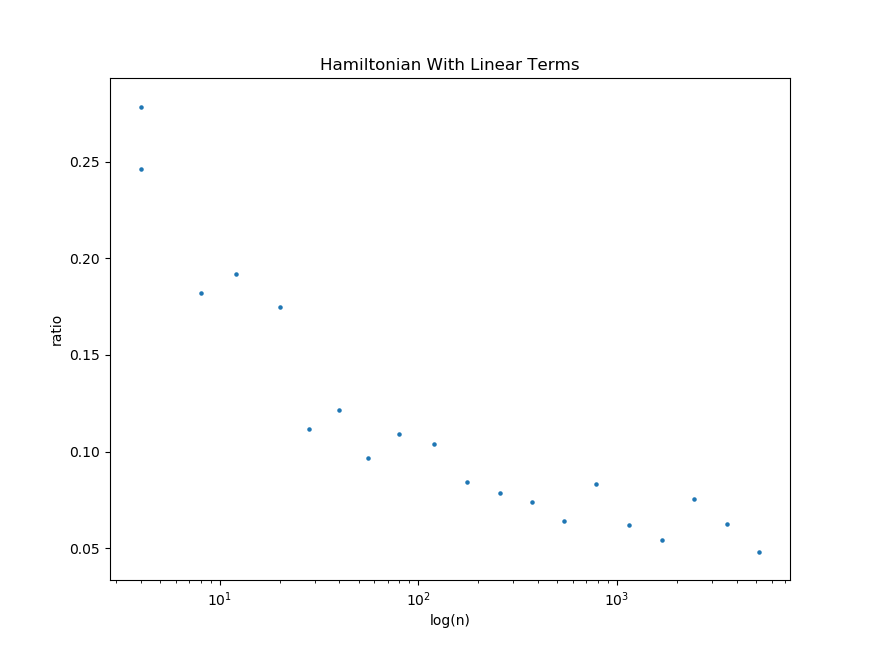
\includegraphics[width=0.9\textwidth]{avgplotn(4,5200,2,20,20)}
	\caption{lalalala}
	\label{fig:avgplotn}
\end{figure}
